\documentclass[titlepage]{jsarticle}                                                                                                                                                                                              

\usepackage{geometry}
\usepackage{bm}
\usepackage{here}
\usepackage{amsmath,amssymb}
\usepackage{ascmac}
\usepackage{siunitx}
\usepackage[dvipdfmx]{graphicx}


\geometry{left=25mm,right=25mm,top=30mm,bottom=30mm}
\begin{document}


\title{大統一模型模型研究ノート}
\author{金沢大学大学院\,\,自然科学研究科数物科学専攻\,(物理学コース)修士課程2年\\学籍番号\,2315011026$\quad$名列番号216\\高村 泰時} 
\date{\today}
\maketitle

\begin{abstract}
  これは修士論文に向けた研究のノートです.
\end{abstract}

\section{素粒子標準模型}
% ---------------------------------------
%
%  Standard model
%  Standard_Model.tex
%  Program modified by Yasutoki Takamura
%  Last Modified Jan 20 2025
%
% ---------------------------------------
この章では素粒子物理学における標準模型についてまとめた.
素粒子標準模型は現在の高エネルギー実験をほぼ説明することができるものであるが, 標準模型だけでは説明できない事実が存在する.
大統一理論はそれらを解決するための理論の一つであるが, そもそも標準模型がどのような理論であるのかをここで振り返る.
\section{概観}
素粒子標準模型は量子場の理論により記述される.
素粒子の相互作用はYang-Millsによる理論によって, 数学的にリー群に属する局所非可換ゲージ変換のもとで不変になるようにラグランジアン密度を記述することができる.
具体的には, 次のようなゲージ対称性を持つ理論である.
\begin{align}
  \mathcal{G}_{\text{SM}}=\mathrm{SU}(3)_\mathrm{c}\times \mathrm{SU}_\mathrm{L}(2)\times \mathrm{U}(1)_\mathrm{Y}\label{SM-Gauge}
\end{align}
それぞれゲージ群の添字は量子数に対応している.
``C''はカラー量子数, ``L''は左巻きのカイラリティ, ``Y''は超電荷である.
$\mathrm{SU}(3)_c$群は核子に作用する強い相互作用を記述する群であり, 量子色力学(QCD)によって記述される.\cite{grossUltravioletBehaviorNonAbelian1973,politzerReliablePerturbativeResults1973a,weinbergNonAbelianGaugeTheories1973}
一方で$\mathrm{SU}(2)_L\times \mathrm{U}(1)_Y$は弱い相互作用と電磁相互作用を統一的に記述する電弱理論を記述する群である.
\cite{glashowPartialsymmetriesWeakInteractions1961,salamWeakElectromagneticInteractions1968,weinbergModelLeptons1967}

ゲージ対称性の他に, 理論に現れる粒子がどのようなものであるのか, 標準模型のゲージ対称性の中でどのような対称性を持つ粒子であるのかを決めることにより, 理論を具体的に決定することができる.
他にも, ラグランジアン密度に含める項は, 繰り込み可能であり, ローレンツ対称性を満足するものを決めることで全て書き下すことができる.
ここからは標準模型に現れる粒子と, その対称性について考える.
\section{ローレンツ代数とスピノール表現}
物質場の基本的な構成をするために, スピノール場を定義する.
スピノール場はローレンツ群$SL(2,\mathbb{C})$の変換をうける.

はじめに, ローレンツ群の表現行列は
\begin{eqnarray}
  D(\Lambda) = \exp\left(-\frac{i}{2\hbar}\omega^{\alpha\beta}S_{\alpha\beta}\right)
\end{eqnarray}
と表される.
$\omega_{\alpha\beta}$は
に対して, 基本表現は
\begin{eqnarray}
  \psi_\alpha' = U_\alpha^\beta \psi_\beta\label{spi_1}
\end{eqnarray}

\section{ゲージ粒子}
量子場の理論は量子力学と特殊相対論を組み合わせたものである.
素粒子の反応を記述することは量子場の理論のみではできないが, ゲージ対称性を理論に課すことにより相互作用を記述することができる.
物質粒子どうしの相互作用を媒介する粒子はゲージ粒子と呼ばれ, スピン$1$のボーズ粒子である.
素粒子標準模型では強い相互作用を媒介するグルーオン($g$), 弱い相互作用を媒介する($W, Z$)ボゾン, 電磁相互作用を記述する光子($\gamma$)がある.
これらはゲージ原理によって理論のラグランジアンに含まれることになる.
\subsection{ゲージ原理}
ゲージ原理とは, 局所変換と呼ばれる時空の各点で独立なゲージ変換を行ったとしても, 物理法則が不変でなければならない主導原理である.

ゲージ粒子は, このゲージ原理によって理論に導入することができる.
先に述べたが, 量子場の理論にゲージ対称性を課すことで相互作用を記述することができる.
この対称性は数学的にリー群によって記述される.
ゲージ原理の一般的な説明のために, 以下では物質場$\Psi(x)$がリー群$G$に属し, $r$重項を成しているとする.

リー群の要素は一般的に$\exp\left(i\sum_{a=1}^n \theta^a T^a\right)$と書かれる.
$\theta^a$は実定数であり, $n=\mathrm{dim}(G)$はリー群の次元である.
ここで, $T^a$はリー群の生成子であり, 交換関係
\begin{align}
  [T^a, T^b] = if_{abc}T^c \label{gauge-1}
\end{align}
を満たす.
ここで$f^{abc}$はリー群の構造定数である.

ここで, ゲージ原理を用いてリー群の対称性によって局所変換のもとで不変な理論を考える.
物質場$\Psi(x)$の局所変換を次のように考える.
\begin{align}
  \Psi(x)\quad\rightarrow\quad\Psi(x)' = \exp\left(i\theta^a(x)T^a(\bm{r})\right)\Psi(x) \equiv U(x)\Psi(x) \label{gauge-2}
\end{align}
このとき, $\theta^a(x)$は積分可能な実関数, $T^a(\bm{r})$は$\bm{r}$次元のリー群の表現行列である.
非可換ゲージ場$A^a_\mu(x)$と共変微分$D_\mu\equiv\partial_\mu+ig A^a_\mu(x)T^a(x)$を導入する
ここで定数$g$はゲージ結合定数である.
この共変微分を導入したことによりゲージ場と物質場の相互作用を記述している.

物質場の共変性からゲージ場の変換を考えることができる.
物質場の共変性は, 局所変換の変換性のもとで
\begin{align}
  D_\mu\Psi(x) \rightarrow D'_\mu \Psi'(x) = U(x) D_\mu \Psi(x)\label{gauge-3}
\end{align}
と変換することである.
このことから, ゲージ場の変換は
\begin{align}
   A_\mu^a(x) T^a(\bm{r}) &\rightarrow A_\mu'^a(x) T^a(\bm{r})\nonumber\\
                          & U(x)A_\mu^a T^a(\bm{r}) U^{-1}(x) -\frac{i}{g}U(x)\partial_\mu U^{-1}(x) \label{gauge-4}
\end{align}
となる.
ここからゲージ場の強さを定義することができる.
共変微分の交換関係は$[D_\mu,D_\nu] = igF_{\mu\nu}^a(x)T^a(\bm{r})$であり, この$F_{\mu\nu}^a$は
\begin{align}
  F_{\mu\nu}^a(x) = \partial_\mu A_\nu^a(x) - \partial_\nu A_\mu^a(x) - gf^{abc}A_\mu^b(x)A_\nu^c(x)\label{gauge-5}
\end{align}
と表され, 場の強さテンソルとして定義される物理量となる.
ここで用いた場の強さテンソル$F_{\mu\nu}^a$は理論のゲージ対称性によりそれぞれ異なる.
非可換ゲージ場のローレンツ不変性とゲージ不変性を要求すると, 運動項は
\begin{align}
  F_{\mu\nu}^a = -\frac{1}{4}F_{\mu\nu}^a F^{a\,\mu\nu}\label{gauge-6}
\end{align}
となる.
ここでは一般的なリー群に基づいたゲージ変換を考えたが, $SU(2), SU(3)$群を考えることで弱い相互作用と強い相互作用を記述することができる.
また, ここで述べたものは非可換ゲージ理論であるが, 電磁相互作用を記述する$U(1)$対称性はこれらの記述を可換なものとして扱えば良い.
その場合, 式(\ref{gauge-5})の第3項は存在しない.
\subsection{ゲージ粒子のラグランジアン}
これまで述べたことを踏まえて, $B_{\mu\nu}$を電磁相互作用を記述する$U(1)$ゲージ場, $W_{\mu\nu}^i\,(i=1,2,3)$を弱い相互作用を記述する$SU(2)$ゲージ場, $G_{\mu\nu}^a\,(a=1,\cdots,8)$を強い相互作用を記述する$SU(3)$ゲージ場とすると, 素粒子標準模型に現れる場の強さテンソルは式(\ref{gauge-5})より次のように表される.
\begin{align}
  B_{\mu\nu} &= \partial_\mu B_\nu - \partial_\nu B_\mu \label{gauge.B}\\
  W_{\mu\nu}^i &= \partial_\mu W_\nu^i - \partial_\nu W_\mu^i+g_2\varepsilon^{ijk}W_\mu^j W_\nu^k \label{gauge.W}\\
  G_{\mu\nu}^a &= \partial_\mu G_\nu^a - \partial_\nu G_\mu^a +g_3 f^{abc}G_\mu^b G_\mu^c\label{gauge.G}
\end{align}
ここでは, $g_3, g_2$はそれぞれ$\mathrm{SU}(3)_\mathrm{c}$, $\mathrm{SU}(2)_\mathrm{L}$ゲージ群の結合定数ある.
また, 後述されるが$\mathrm{U(1)}_{\mathrm {Y}}$ゲージ場によって現れる$B_\mu$ゲージボゾンの結合定数を$g'$とする.
$f^{abc}, \varepsilon_{ijk} $はそれぞれの構造定数を表す.
また, 標準模型のゲージ場の運動項は式(\ref{gauge-6})より
\begin{align}
  \mathcal{L}_{\text{gauge}} = -\frac{1}{4}B_{\mu\nu} B^{\mu\nu} - \frac{1}{4}W_{\mu\nu}^i W^{i\mu\nu} -\frac{1}{4}G_{\mu\nu}^i G^{i\mu\nu}\label{gauge.kin}
\end{align}
と表せる.
\section{フェルミオン}
標準模型粒子ではクォーク, レプトンは物質粒子という枠組みで説明され, スピンが$\frac{1}{2}$のフェルミ粒子である.

標準模型では物質粒子は世代と呼ばれる構造をもつ.
現在の標準模型は3世代模型として考えられており, 弱い相互作用でのCP対称性の破れに重要な役割を果たす.[]

物質粒子はカイラリティと呼ばれる右巻き粒子と左巻き粒子の状態によって区別される.
\textcolor{red}{カイラリティの説明をするべきか?}
\section{ヒッグス機構}
標準模型はゲージ対称性により記述される理論で大きな成功をおさめた.
ところが, この対称性が破れない場合, 次のような問題が残る.
\begin{itemize}
  \item 短距離力である弱い相互作用を記述するゲージボゾンは質量を持つ必要がある. ところがゲージボゾンが局所対称性を維持してしまうと, 質量を持つ項を書くことができない.
  \item クォークやレプトンの質量項を考えると, 右巻きフェルミオンは$SU(2)_L$一重項に属するため, ゲージ不変な質量項を書くことが許されない.
\end{itemize}
これらの問題を解決するためにはゲージ対称性を自発的に破る必要がある.

素粒子標準模型において, ヒッグス場は$SU(2)_L$の複素二重項として次のように書く.
\begin{align}
  \Phi(x) = \left(
  \begin{array}{c}
    \phi^+ \\
    \phi^0
  \end{array}
  \right)
\end{align}
ヒッグス場のラグランジアン密度は
\begin{align}
  \mathcal{L}_H = \left(D_\mu \Phi\right)^\dagger (D^\mu \Phi) -V(\Phi) \label{L_H}
\end{align}
となる.
第2項はヒッグス場のスカラーポテンシャルであり,
\begin{align}
  V(\Phi) = -\mu^2 (\Phi^\dagger\Phi)+ {\lambda}(\Phi^\dagger \Phi)^2,\quad(\mu^2, \lambda>0)\label{V_H}
\end{align}
である.
ヒッグス場のポテンシャルは
\begin{align}
  (\Phi^\dagger \Phi) = \frac{\mu^2}{2\lambda}\nonumber
\end{align}
のときに最小の値をとる.
真空期待値は一般的に
\begin{align}
  \langle 0 |\Phi |0\rangle = \frac{1}{\sqrt{2}}\left(\begin{array}{c}
      0 \\
      v
  \end{array}\right)\label{Higgs_VEV}
\end{align}
のように取ることができるので, 真空期待値は
\begin{align}
  v^2 = \frac{\mu^2}{\lambda}\nonumber
\end{align}
となる.

ヒッグス場を真空期待値の周りで次のように展開する
\begin{align}
  \Phi(x) = \exp\left(i\frac{\pi(x)}{v}\right)\left(
  \begin{array}{c}
    0 \\
    \cfrac{1}{\sqrt{2}}\left(v + h(x)\right)
  \end{array}
\right),\quad \left(\pi(x) = \sum_{a=1}^3\pi^a(x)\frac{\sigma^a}{2}\right)\label{higgs}
\end{align}
ただし, $\pi(x)$は南部・ゴールドストンボゾンであり, ユニタリーゲージを取るとゲージ変換で取り除くことができる非物理的自由度である.
一方で, $h(x)$が実ヒッグス粒子として考えられる.
$\pi^a(x),\,(a=1,2,3)$の3つの自由度のうち,  2つが$W^\pm$ボゾンに吸収され, 1つが$Z^0$ボゾンに吸収されることで, それぞれのゲージボゾンが質量を獲得する.

ここから, ゲージ粒子の質量の獲得について考える.
ヒッグス場のラグランジアン密度は式(\ref{L_H})で与えられており, ヒッグス粒子の運動項には
\begin{align}
  \mathcal{L}_H \supset \frac{1}{4}\left((g_2W^a_\mu\frac{\sigma^a}{2}+g'B_\mu)\Phi\right)^\dagger \left((g_2W^{a\,\mu}\frac{\sigma^a}{2}+g'B^\mu)\Phi\right)\label{eq2-18}
\end{align}
という項が含まれている.
ここで$g'$は$U(1)_Y$ゲージボゾン$B_\mu$のゲージ結合定数である.
これによりゲージ対称性は
\begin{align}
  SU(3)_c\times SU(2)_L\times U(1)_Y \rightarrow SU(3)_c\times U(1)_{em}
\end{align}
のように自発的に破れる.
したがって, (\ref{eq2-18})から
\begin{align}
  \mathcal{L}_H \supset \frac{v^2}{8}\left[\left(g_2^2(W^1_\mu  W^{1\mu}+W^2_\mu  W^{2\mu}\right)+ (g_2W_\mu^3 -g'B_\mu)(g_2W^{3\mu}-g' B^{\mu})\right] \label{2-21}
\end{align}
となる.
ここで, ゲージ場$W_\mu^a$と$B_\mu$を次の様に再定義する.
\begin{align}
  W_\mu^\pm &= \frac{1}{\sqrt{2}}(W_\mu ^1 \mp i W_\mu^2)\\
  \left(\begin{array}{c}
      Z_\mu^0 \\
      A_\mu
      \end{array}\right)&=\frac{1}{\sqrt{g'^2+g_2^2}}\left(\begin{array}{c}
      g_2 W_\mu^3-g' B_\mu \\
      g' W_\mu^3-g_2 B_\mu 
    \end{array}\right)
    \equiv \left(\begin{array}{cc}
        \cos\theta_W W_\mu^3 - \sin\theta_W B_\mu \\
        \sin\theta_W W_\mu^3 + \cos\theta_W B_\mu
      \end{array}
    \right)\label{eq2-22}
\end{align}
ただし, この混合角$\theta_W$は
\begin{align}
  \cos\theta_W = \frac{g_2}{\sqrt{g'^2 + g_2^2}},\quad \sin\theta_W = \frac{g'}{\sqrt{g'^2 + g_2^2}}\nonumber
\end{align}
で定義され, ワインバーグ角と呼ばれる.
実験によりこの値は$\sin^2\theta_W \simeq 0.23$となる.
式(\ref{2-21})から$W^\pm$ボゾンと$Z^0$ボゾンの質量は
\begin{align}
  m_W^2 W_\mu^+W^{-\mu} + \frac{1}{2}\left(\begin{array}{cc}
      A_\mu & Z_\mu
    \end{array}\right) \left(\begin{array}{cc}
      0 & 0 \\
      0 & m_Z^2 
      \end{array}\right)\left(\begin{array}{c}
      A^\mu \\
      Z^\mu
  \end{array}\right)\label{eq2-23}
\end{align}
さらに,
\begin{align}
  m_W = \frac{1}{2}g_2v,\quad m_Z = \frac{1}{2}\sqrt{g'^2+g_2^2}v\nonumber
\end{align}
となる.
これらも質量は
\begin{align}
  m_W \simeq 80.4\,\mathrm{[GeV]},\qquad m_Z \simeq 91.2\,\mathrm{[GeV]} \nonumber
\end{align}
と観測されている.
また, 式(\ref{eq2-22}), (\ref{eq2-23})に表れる$A_\mu$は質量がないことがわかり, $U(1)_{em}$ゲージ場の相互作用をする光子であることがわかる.

ヒッグス場の真空期待値の値は, 4体フェルミ相互作用の観測によって, フェルミ結合定数$(G_F\simeq 1.166\times 10^{-5}\,\mathrm{[GeV]}^{-2})$から導かれた.
場の理論の計算によれば
\begin{align}
  2\sqrt{2}G_F = \frac{g_2^2}{2m_W^2} = \frac{2}{v^2}\nonumber
\end{align}
と与えられるので, $v \simeq 246\,\mathrm{[GeV]}$と定めることができる.
2012年に発見されたヒッグス粒子は$h(x)$であると考えられており, その質量は$m_H = \sqrt{2\lambda}v \simeq 125\,\mathrm{[GeV]}$と明らかになり, ヒッグス場の結合定数が$\lambda \simeq 0.13$と決まった.
% ----- フェルミオン質量の獲得 -----
\section{フェルミオン質量の獲得}
素粒子標準模型において, クォークやレプトンは3つの世代構造を持ち, 右巻き及び左巻きの2つのカイラリティを持つ.
フェルミオンの質量はディラック質量項で書かれる.
ディラックフェルミオン$\psi$をカイラルフェルミオン($\psi_L, \psi_R$)として$\psi=\psi_L + \psi_R$と分解して考える.
フェルミオンの質量項は
\begin{align}
  \mathcal{L}_{\mathrm{Mass}} = -m\bar{\psi}\psi = -m(\bar{\psi}_R\psi_L + \bar{\psi}_L\psi_R)\nonumber
\end{align}
と書かれる.
一方で, カイラリティが左巻きのフェルミオンは$SU(2)_L$二重項である一方, 右巻きのフェルミオンは$SU(2)_R$一重項であるため, その積は$SU(2)_L$変換の下で不変ではない.
そのためラグランジアンに含めることは許されない.

ヒッグス場によってゲージ対称性を破ることが説明され, ゲージボゾンのみならずクォークやレプトンに対しても質量を与えることが可能となる.
$i=1,2,3$を世代数として, 図\ref{fig_sm}のようにまとめられる.
\begin{table}[ht]
  \caption{標準模型粒子と量子数}
  \begin{center}
    \begin{tabular}{cc|cc}\hline
  クォーク場 & 量子数 & レプトン場 & 量子数 \\\hline\hline
  $Q_i\equiv\begin{pmatrix}
    u_i \\
    d_i
  \end{pmatrix}_{L}$
 & $\left(\bm{3}, \bm{2}, \cfrac{1}{6}\right)$ &  $L_i\equiv\begin{pmatrix}
    \nu_{li} \\
    l_i
  \end{pmatrix}_{L}$ & $\left(1,\bm{2},-\cfrac{1}{2}\right)$ \\
  $u_{iR}$ & $\left(\bm{3},1,\cfrac{2}{3}\right)$ & $l_{iR}$ & (1,1,-1) \\
  $d_{iR}$ & $\left(\bm{3},1,-\cfrac{1}{3}\right)$ & & \\\hline
  \label{fig_sm}
    \end{tabular}
  \end{center}
\end{table}
\subsection{レプトン場の質量生成}
はじめにレプトンの質量について考える.
レプトン場とヒッグス場からなる$\mathcal{G}_{\mathrm{SM}}$不変な湯川相互作用は
\begin{align}
  \mathcal{L}_Y \supset -Y_{l}^{ij} \overline{L_i}\Phi l_{jR} +\mathrm{h.c.}
\end{align}
と表される.
ヒッグス場が真空期待値を(\ref{Higgs_VEV})のようにとると質量項を書くことができる.
\begin{align}
  \mathcal{L}_{Mass} \supset -m_e\bar{e}e -m_\mu \bar{\mu} \mu - m_\tau \bar{\tau}\tau\nonumber
\end{align}
\begin{align}
  M_l = Y_l\frac{v}{\sqrt{2}}
\end{align}
\subsection{クォーク場の質量生成}
クォーク場とヒッグス場からなる$\mathcal{G}_{\mathrm{SM}}$不変な湯川相互作用は
\begin{align}
  \mathcal{L}_Y \supset -Y_{d}^{ij} \overline{Q_i}\Phi d_{jR} -Y_{u}^{ij} \overline{Q_i}i\sigma^2\Phi u_{iR} +\mathrm{h.c.}
\end{align}
と表せる.

\section{走るゲージ結合定数}
場の量子論に基づけば, 理論に現れる発散を繰り込みという手法を用いて取り除くことが可能である.
\textcolor{red}{種類などもう少し細かい説明をするか?}

いずれの方法であってもエネルギースケールへ依存性があるが, 理論はエネルギーの変化に対して不変でなければならないため, ラグランジアンに存在するパラメータはエネルギースケールの変化を打ち消すように変化する.
これによってエネルギースケールに依存する繰り込まれた理論が得られる.
\subsection{Callan-Symanzik方程式}
繰り込まれた量子場の理論ではラグランジアンの項は制限が与えられ, 質量次元が4次の項のみ許される.
繰り込まれた場の理論のパラメータは, 繰り込み条件の組みで決定され, この条件が繰り込みスケールを決定している.
異なるエネルギースケールであっても同様の理論を考えることができる.

繰り込み条件を考えると, 繰り込みを行うスケール$M$は任意である.
したがって, 同じ理論を異なったスケール$M'$でも定義することができる.
このことを以下で考える. 

ある理論のグリーン関数が
\begin{align}
  \langle T \phi_0(x_1)\cdots\phi_0(x_n)\rangle  \label{rescale1}
\end{align}
で与えられるとする.
この理論では, 量子効果を考えない裸の結合定数$\lambda_0$や, 運動量カットオフが$\Lambda$によって与えられるものであり,エネルギースケール$M$には依存していない.
エネルギースケール依存性は, このグリーン関数にあるのではなく, 場をリスケーリングし裸の結合定数$\lambda_0$を消して繰り込まれた結合定数$\lambda$で書くことでカットオフ依存性を取り除いたときにのみ現れる.
繰り込まれたグリーン関数と裸のグリーン関数は, リスケーリング因子の$Z$に至るまでは数値的に同じになる.
場の繰り込みは場の強さの繰り込み因子である$Z$を用いて次のように定義される.
\begin{align}
  \phi(x) = Z^{-\frac{1}{2}}\phi_0(x) \label{bfnc-2}
\end{align}
これにより繰り込まれた$n$点の相関関数は, 裸の相関関数と次のように関係付けられる.
\begin{align}
  \langle T \phi(x_1)\cdots \phi(x_n)\rangle = Z^{-\frac{n}{2}}\langle T \phi_0(x_1)\cdots \phi(x_n)\rangle \label{bfnc-1}
\end{align}
式(\ref{bfnc-1})の左辺は繰り込まれたグリーン関数と呼ばれる.
この関数は右辺のグリーン関数とは異なる別のエネルギースケールである$M'$で定義されており, 結合定数は$\lambda'$, リスケーリング因子は$Z'$で定義される.

ここから, エネルギースケール$M$を無限小だけシフトした場合の影響を考える.
はじめに$G^{(n)}(x_1,\cdots,x_n)$を繰り込まれた摂動論において計算される連結$n$点関数とする.
\begin{align}
  G^{(n)}(x_1,\cdots,x_n) = \langle T\phi(x_1)\cdots\phi(x_n) \rangle_{\text{connected}}\label{rnpf}
\end{align}
繰り込みされていない裸の相関関数は, 繰り込みされていないパラメータである$(\phi_0,\lambda_0,m_0)$とカットオフ$\Lambda$に依存している.
一方で, 繰り込まれた相関関数(式(\ref{rnpf}))には繰り込まれたパラメーターである($\phi,\lambda,m)$と繰り込みスケール$M$に依存している.
このことから, 繰り込みされていない裸の相関関数$G^{(n)}_0$は繰り込みスケール$M$に依存せず, 繰り込みスケールの変化があった場合でも変化することがないので
\begin{align}
  \frac{d G_0^{(n)}}{dM} = 0 \label{bfnc-3}
\end{align}
が満たされる.
一方で, 繰り込まれた相関関数は繰り込みスケールが変化することで影響を受ける.
繰り込みスケールを無限小だけシフトする.
\begin{align}
  M\quad\rightarrow\quad M + \delta M \label{sftM}
\end{align}
このとき, 繰り込みスケールの変化に伴って$\lambda$と$\phi$は次のように変化する.
\begin{align}
  &\lambda \quad\rightarrow\quad \lambda + \delta \lambda \label{sftl}\\
  &\phi \quad\rightarrow\quad \phi+ \delta\phi \equiv (1+\delta\eta)\phi \label{sftp}
\end{align}
場の変換については無次元のシフトを$\delta \eta  = \frac{\delta\phi}{\phi}$とした.
式(\ref{bfnc-2})から
\begin{align}
  Z^{\frac{1}{2}} = 1 - \delta\eta\label{bfnc-4}
\end{align}
が言えるので, 式(\ref{bfnc-3})から繰り込みされた相関関数は
\begin{align}
  G^{(n)}\quad\rightarrow\quad(1+n\delta\eta)G^{(n)}\label{sftg}
\end{align}
と変化することがわかる.
これらを踏まえて, 繰り込みされた相関関数の微小変化を考えると, 式(\ref{bfnc-3})から
\begin{align}
  \frac{d}{dM} Z^{\frac{n}{2}}G^{(n)} = \frac{\partial G^{(n)}}{\partial M} + \frac{\partial G^{(n)}}{\partial \lambda}\frac{\partial \lambda}{\partial M} - n \frac{\partial \eta}{\partial M}G^{(n)} = 0
\end{align}
がわかるので, これを整理して
\begin{align}
  \left(M \frac{\partial}{\partial M} + M\frac{\partial \lambda}{\partial M} \frac{\partial}{\partial \lambda} -nM\frac{\partial \eta}{\partial M}\right)G^{(n)}(x_1,\cdots,x_n;M,\lambda) = 0\label{CS-1}
\end{align}
となる.
ここで無次元の量である$\beta$と$\gamma$を
\begin{align}
  &\beta = M\frac{\partial \lambda}{\partial M}\label{def_beta}\\
  &\gamma = -M\frac{\partial \eta}{\partial M} \label{def_gamma}
\end{align}
と定義すると, 次の関係式が得られる.
\begin{align}
  \left(M \frac{\partial }{\partial M} + \beta \frac{\partial}{\partial \lambda} + n \gamma\right) G^{(n)}(x_1,\cdots,x_n;M,\lambda) = 0 \label{bfnc-CS1}
\end{align}
式(\ref{bfnc-CS1})はCallan-Symanzik方程式と呼ばれる. \cite{callanBrokenScaleInvariance1970,symanzikSmallDistanceBehaviour1970,symanzikSmalldistancebehaviourAnalysisWilson1971}

Callan-Symanzik方程式に現れる$\beta, \gamma$の2つの関数はカットオフスケールの$\Lambda$に依存し, 繰り込みスケール$M$に依存しない.
つまり, この$\beta, \gamma$の2つの関数は次元を持たない繰り込まれた結合定数である$\lambda$の関数であることが言える.
これらは$G^{(n)}$にのみ繰り込みが行われているからである.

ここで新しく定義された$\beta, \gamma$の2つの関数は不変的な関数であり, 繰り込み定数と場の強さの変化にのみ依存しており, これらが変化したときの繰り込みスケール$M$の変化を補うように変化が起こる. 
そのため$\beta$関数は繰り込みスケールが$M$への結合定数の依存性を表し, 一方で$\gamma$関数は場を繰り込みスケール$M$への依存性を表している

次にCallan-Symanzik方程式に現れた新たな関数$\gamma$をを一般化し, 摂動との関係を考える.
$\delta \eta$は式(\ref{sftp})で定義されていた.
したがって,
\begin{align}
  \delta \eta &= \frac{Z^{-\frac{1}{2}}(M+\delta M)}{Z^{-\frac{1}{2}}(M)}-1\nonumber\\
              &= \frac{Z^{-\frac{1}{2}}(M+\delta M)-Z^{-\frac{1}{2}}(M)}{Z^{-\frac{1}{2}}(M)}
\end{align}
となる.
この両辺を$\delta \mu$で割り, $\delta \mu\rightarrow0$とすると
\begin{align}
  \frac{\partial \eta}{\partial M} = -\frac{1}{2}\frac{1}{Z}\frac{\partial Z}{\partial M}
\end{align}
一方で$\gamma$は式(\ref{def_gamma})で定義されているので,
\begin{align}
  \gamma = \frac{1}{2}\frac{M}{Z} \frac{\partial Z}{\partial M}\label{def_gamma_correct}
\end{align}
と$\gamma$の表し方を変えることができる.
ここから摂動論の関係を見ることができる.
摂動論を考えているとき, 場の強さ$Z$は
\begin{align}
  Z = 1 +\delta Z
\end{align}
と微小量$\delta Z \ll 1$を用いて書くことができる.
これより
\begin{align}
  \gamma \simeq \frac{1}{2}M \frac{\partial \delta Z}{\partial M} + \mathcal{O}((\delta Z)^2)
\end{align}
となる.
このことから摂動論が有効な理論であれば, $\delta Z$が判明すれば 相殺項から体系的に$\beta$関数を求めることができることがわかる.

ここまではCallan-Symanzik方程式をスカラー場の理論として式(\ref{rescale1})から導出した.
一般にフェルミオン場が存在した場合でも成り立つ.
$n$個のフェルミオン場, $m$個のスカラー場が存在し, 両方の結合定数が$\lambda$の場合を考える.
このとき, 場のくりこみを同じように考えると, 繰り込まれたグリーン関数は
\begin{align}
  G_0^{(n,m)}(\{x_i\},\lambda_0) = Z_\psi^{\frac{n}{2}} Z_\phi^{\frac{m}{2}}G^{(n,m)}(\{x_i\},\lambda,M)\label{renormalized_G}
\end{align}
となる.
したがって, 式(\ref{bfnc-3})と同じように考えて
\begin{align}
  \left(M\frac{\partial}{\partial M} + \beta\frac{\partial}{\partial \lambda} + n\gamma_\psi + m \gamma_\phi \right)G^{(n,m)}(\{x_i\},M,\lambda) = 0\label{renormalized_CS}
\end{align}
となる.
ここでは
\begin{align}
  \gamma_\psi = \frac{n}{2}\frac{M}{Z_\psi}\frac{\partial Z_\psi}{\partial M},\quad \gamma_\phi = \frac{m}{2}\frac{M}{Z_\phi}\frac{\partial Z_\phi}{\partial M}\label{def_gamma2}
\end{align}
とした.

これらより, 式(\ref{def_beta})
\begin{align}
  \beta \equiv M\frac{\partial}{\partial M}\lambda\nonumber
\end{align}
の$\beta$からゲージ結合定数$\lambda$のエネルギー依存性を求めることができる.
この$\beta$は摂動論において相殺項や繰り込まれたグリーン関数から求めることができ, 非可換ゲージ理論や湯川結合, スカラー場の理論など一般的な場の理論で同様に求めることができる.
\cite{chengHiggsPhenomenaAsymptotically1974,
machacekFermionHiggsMasses1981,
machacekTwoloopRenormalizationGroup1983,
machacekTwoloopRenormalizationGroup1984,
machacekTwoloopRenormalizationGroup1985,
maVariationMixingAngles1979,
vaughnRenormalizationGroupConstraints1982}
\subsection{ゲージ結合定数のエネルギー依存性}
式(\ref{def_beta})により, ゲージ結合定数のエネルギー依存性を$\beta$関数によって導くことができることが明らかにされた.
理論に現れる相殺項を求めることで$\beta$-関数の具体的な形を求めることができるが, 群論の対称性を用いることで一般的な$\beta$-関数の係数は導出されている.
摂動の$\delta Z$の1次の影響まで考えた場合,
\begin{align}
  \beta = -\frac{g^3}{(4\pi)^2}\left[\frac{11}{3}C_2(G) -\frac{4}{3}\kappa S_2(F) - \frac{1}{6}\eta S_2(S)\right]
\end{align}
となる.\cite{grossUltravioletBehaviorNonAbelian1973,politzerReliablePerturbativeResults1973b}
\footnote{
本論文では扱わないが, 2次までの摂動の計算をすると次のようになる.
\cite{caswellAsymptoticBehaviorNonAbelian1974,jonesTwoloopDiagramsYangMills1974}
\begin{align}
  \beta &= -\frac{g^3}{(4\pi)^2}\left[\frac{11}{3}C_2(G) -\frac{4}{3}\kappa S_2(F) - \frac{1}{6}\eta S_2(S)\right] \nonumber\\
        &\quad-\frac{g^5}{(4\pi)^4}\left[ \frac{34}{3}[C_2(G)]^2 -\kappa\left(4C_2(F)+\frac{20}{3}C_2(G)\right)S_2(F) -\left(2C_2(S)+\frac{1}{3}C_2(G)\right)\eta S_2(S)\right] \nonumber
\end{align}
}

\begin{figure}[ht]
  \centering
  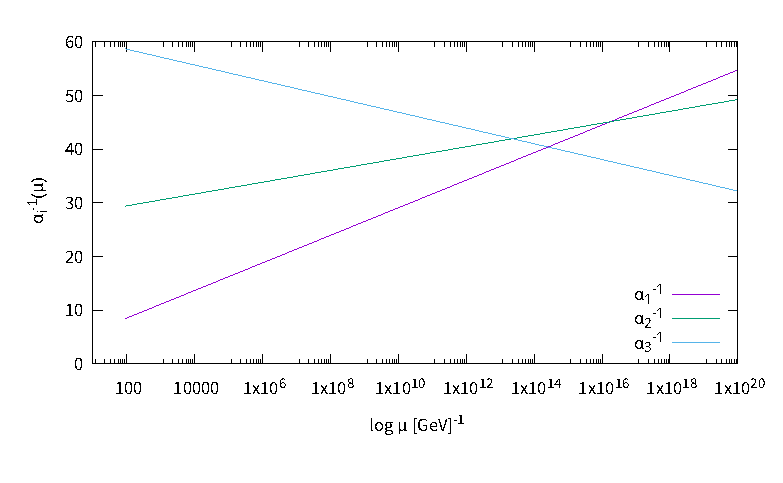
\includegraphics[width=12truecm,clip]{fig/RGE_SM.eps}
  \caption{標準模型粒子のみで繰り込み群方程式を解いた図}
  \label{fig:RGE_SM}
\end{figure}
%EOF



\end{document}

